\documentclass{article}
\usepackage{graphicx} % Required for inserting images
\usepackage{amsmath}
\usepackage{physics,amsmath}
\usepackage{float}
\usepackage{hyperref}

\hypersetup{colorlinks=true, urlcolor=cyan, linkcolor=black}

\title{Protons in the Earth's Magnetic Field}
\author{Ingve Aleksander Hetland}
\date{March 2023}

\begin{document}

\maketitle

\section{Abstract}
In order to study how charged particles from solar winds interact with the magnetic field of the earth, as seen especially during events of northern lights, we model the earth's magnetic field as that of a pure dipole and numerically solve the equations of motion for incoming charged particles in this field. We then present plots of the trajectories of particles with varying initial conditions, and discuss the nature of the trajectories and how they change with initial conditions. Lastly we discuss the relevance of our findings in the case of actual solar winds.

\section{Introduction}
As my mother and I were taking a stroll that fateful Christmas night, I indeed immediately began my work to simulate the particle trajectories of the northern lights. Thankfully, the embarrassment of not knowing how they looked was to be short lived, because the plots I produced were as beautiful as they were fascinating. Though my mother did not think the trajectories made sense, I, the unseasoned physicist, stood astonished in the woods watching my Jupyter plots while my mother was shivering from the dreadful cold.\\
\\
I will in this report present a model for the earth's magnetic field and numerical calculations of the trajectories for moving particles in this field. This very simplified model will serve to give insight into how particles in solar winds move under the influence of the earth's magnetic field, and hence some of the mechanisms of the northern lights. The analysis consists of testing different initial conditions for the particles, as well as testing different orientations of the earth's magnetic field, as it would vary throughout the year whilst rotating around the sun. Lastly I discuss different aspects of the results, such as how initial position, initial velocity, and orientation of the field change the path of the particles and discuss the accuracy of my results.

\section{Theory}
The earth's magnetic field behaves to a good approximation like a pure magnetic dipole located at the center of the earth. The magnetic field of a pure dipole is given by

\begin{equation}
    \boldsymbol{B}_{dip}(\boldsymbol{r}) = \frac{\mu_0}{4\pi}\frac{\boldsymbol{m}\cross\boldsymbol{r}}{r^3}
\label{eq:dipoleField}
\end{equation}
\\
where $\mu_0$ is the magnetic permeability of free space, $\boldsymbol{m}$ is the magnetic dipole moment, $\boldsymbol{r}$ is the position vector, and $r = \abs{\boldsymbol{r}}$.\\
\\
For a particle with charge $q$ and mass $m$ which is moving with a velocity $\boldsymbol{v}$ in electromagnetic fields $\boldsymbol{E}$ and $\boldsymbol{B}$, the force on the particle from is given by the Lorentz force

\begin{equation}
    \boldsymbol{F}=q(\boldsymbol{E}+\boldsymbol{v} \cross\boldsymbol{B})
\label{eq:LorentzForce}
\end{equation}
\\
An important note about the Lorentz force due to the magnetic field is that the cross product between the velocity and the magnetic field ensures that the force always acts perpendicular to the direction of motion. This in turn means that the magnetic field does not do any work on the particle.\\

By Newton's second law, the acceleration of such a particle due to the electromagnetic fields is given as

\begin{equation}
    \boldsymbol{a}=\frac{q}{m}(\boldsymbol{E}+\boldsymbol{v} \cross\boldsymbol{B})
\label{eq:acceleration}
\end{equation}
\\
I have found it convenient to introduce a rotation matrix $\underline{R}$ that rotates a 3-dimensional column vector $\boldsymbol{v}$ arbitrarily through three consecutive rotations by the transformation

\begin{equation}
    \boldsymbol{v}' = \underline{R}\boldsymbol{v}
\label{eq:Rotation}
\end{equation}
where $\underline{R}$ is the $3\cross3$ rotation matrix

\begin{equation}
    \underline{R}=\left(\begin{matrix}
    c_1c_3-c_2s_1s_3 & -c_1s_3-c_2c_3s_1 & s_1s_2 \\
    c_3s_1+c_1c_2s_3 & c_1c_2c_3-s_1s_3 & c_1s_2 \\
    s_2s_3 & c_3s_2 & c_2
    \end{matrix}\right)
\label{eq:defineR}
\end{equation}
\\
"$c$" refers to a cosine and "$s$" to sine. {$1,2,3$} refers to the Euler angles {$\alpha,\beta,\gamma$} respectively. $\underline{R}$ denotes specifically a $zxz$-rotation; meaning we rotate $\alpha$ degrees about the $z$-axis, then $\beta$ degrees about the $x$-axis, and finally $\gamma$ degrees about the $z$-axis. 

\section{Methods}
We define a coordinate system where the center of the earth is located at the origin. The sun will in this system lie at some point in the negative $x$-direction, meaning the eventual solar wind particles will move from negative to positive $x$. The $z$-direction is defined to be perpendicular to the ecliptic of the sun and earth.\\
\\
For the calculations it was convenient to define a unit system with typical magnitudes that we are working with, such that the quantities can be made dimensionless. These characteristic magnitudes are largely based upon the earth's radius, the elementary charge, the proton mass, and typical speeds of solar winds. The quantities are are summarized in Table \ref{tab:characteristicMagnitudes}.

\begin{table}[h]
    \centering
    \begin{tabular}{c|c|c|c}
        Quantity & Symbol & Value & Unit\\
        Mass & $m_p$ & $1.67\cdot10^{-27}$ & kg \\
        Charge & $q_0$ & $1.60\cdot10^{-19}$ & C \\
        Time & $t_0$ & $14.2$ & s \\
        Distance & $R_0$ & $6.37\cdot 10^{6}$ & m \\
        Speed & $v_0$ & $4.47\cdot10^4$ & m/s \\
        Magnetic Dipole Moment & $m_0$ & $1.93\cdot10^{19}$ & J/T \\
        Magnetic Field & $B_0$ & $7.37\cdot10^{-9}$ & T
    \end{tabular}
    \caption{Characteristic magnitudes of quantities which are used in the calculations}
    \label{tab:characteristicMagnitudes}
\end{table}

\noindent In order to plot the magnetic field of the dipole I implemented eq. \ref{eq:dipoleField} as a function, defined coordinate arrays in 3 dimensions and defined the magnetic dipole moment of the system as $\boldsymbol{m}/m_0$ in the negative $z$-direction. Since the earth is tilted by about $11^{\circ}$ with respect to the $z$-axis, we rotate our dipole moment using the transformation defined by eq. \ref{eq:Rotation}, using $\beta=11^{\circ}$. Since we have defined a general way of rotating a vector, we can investigate how solar wind particles will move at different times of the year by tweaking the angle $\alpha$. 

\section{Results}
We constructed a discrete coordinate system ranging from $-5R_0$ to $5R_0$ along each coordinate axis divided into $7\cross 7\cross 7$ coordinate points, and calculated the magnetic field of a dipole at the origin in these points using our implementation of eq. \ref{eq:dipoleField}. The resulting field with the corresponding dipole moment is presented in 3D in Figure \ref{fig:dipoleField}, and the planes through the origin are plotted in 2D in Figure \ref{fig:dipolePlanes}\\

\begin{figure}[H]
    \centering
    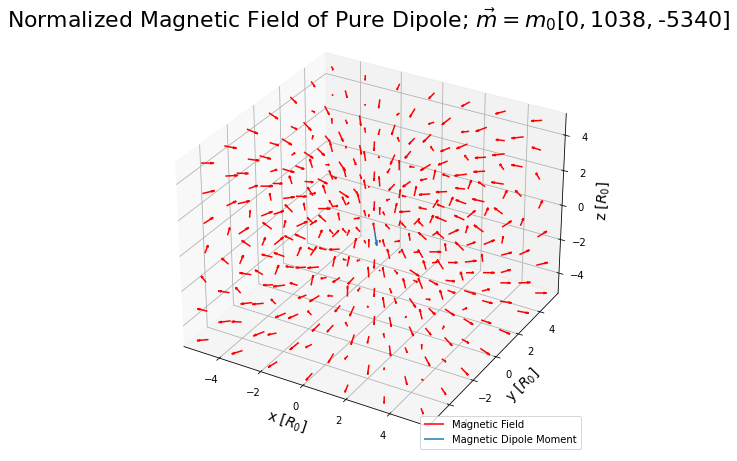
\includegraphics[scale=.4]{Images/dipoleField.png}
    \caption{Plot of the magnetic field of a pure dipole without magnitude and its corresponding magnetic dipole moment.}
    \label{fig:dipoleField}
\end{figure}

\noindent It can be observed in Figure \ref{fig:dipoleField} that the dipole field has azimuthal symmetry around an axis along the dipole moment and that the field lines point from the magnetic north to the magnetic south, which is exactly how a magnetic dipole behaves. This plot does not portray strength, only direction.\\
\\
We study the field further by assessing the $xz$-plane and $yz$-plane through the origin in shown in Figure \ref{fig:dipolePlanes}. Since the differences in magnetic field strength vary a lot with distance from the source, the strength in Figure \ref{fig:dipolePlanes} has been cut off at $1000B_0$, meaning differences near the center are not discernible.\\

\begin{figure}[H]
    \centering
    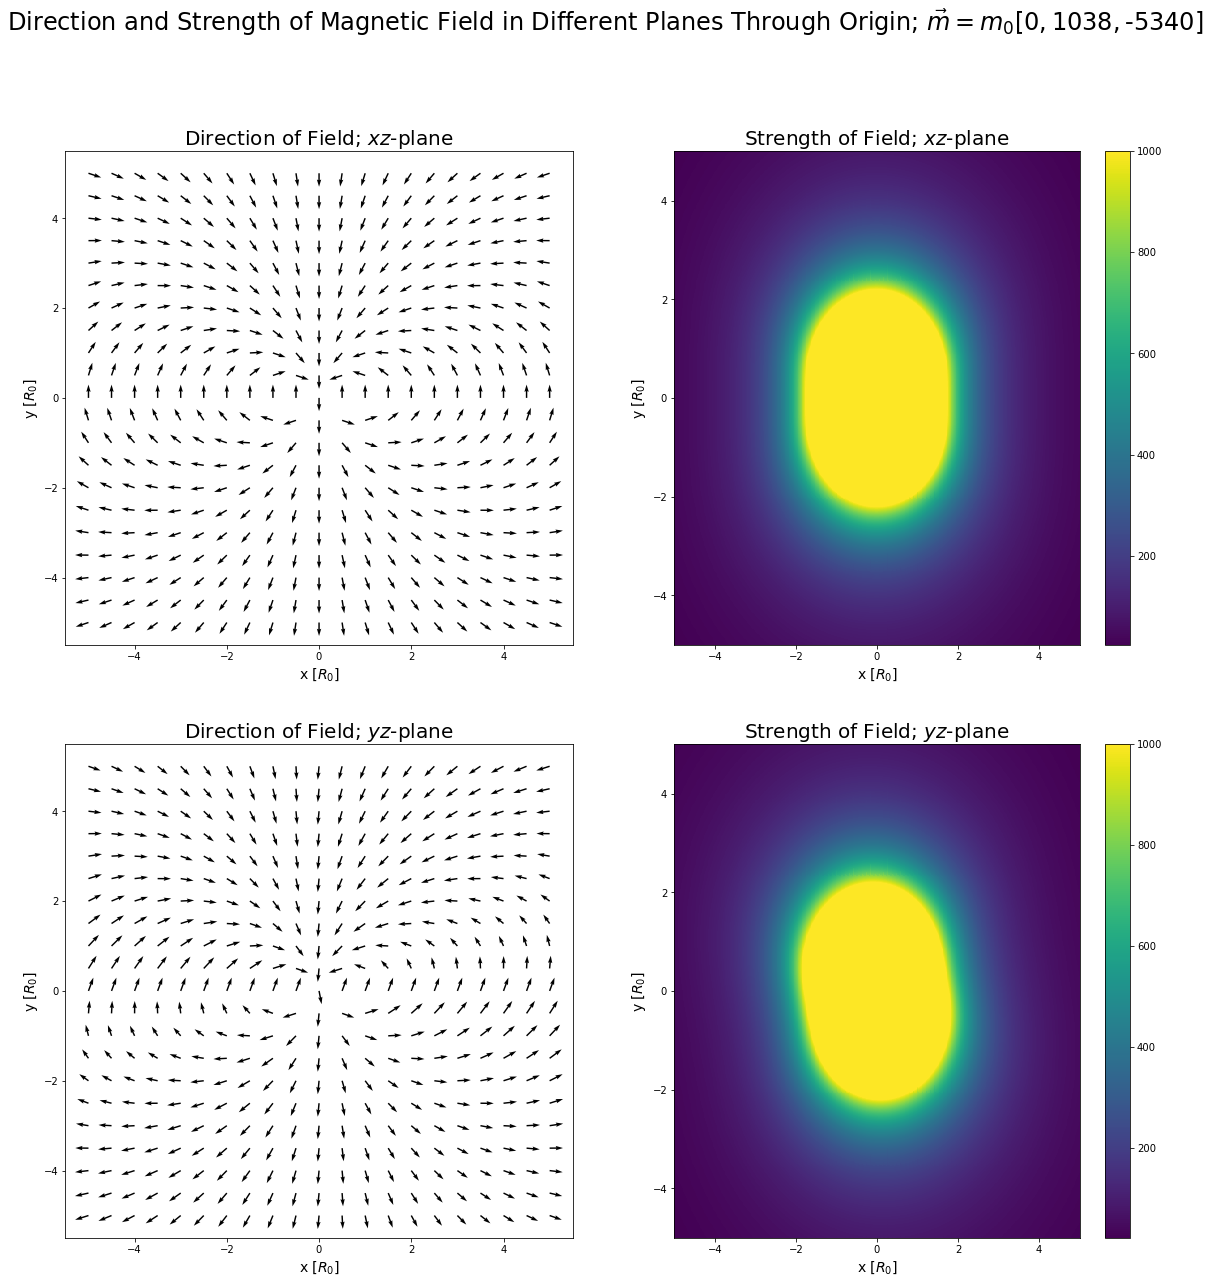
\includegraphics[scale=.28]{Images/dipolePlanes.png}
    \caption{Direction and strength of the magnetic field of our dipole in the $xz$-plane (upper images) and in the $yz$-plane (lower images).}
    \label{fig:dipolePlanes}
\end{figure}

\noindent Most apparent is the fact that the magnetic field is tilted in the $yz$-plane, which corresponds to the tilt we imposed on our dipole moment. This tilt can also be seen in Figure \ref{fig:dipoleField}, though it is harder to see. A note about Figure \ref{fig:dipolePlanes} is that the strength of the field, though exaggerated in the plots, has an elliptical shape along the dipole moment. This corresponds to the real behaviour of a dipole.\\
\\
We now turn our attention to the trajectory for a proton travelling through the earth's magnetic field, for which the plots in figures \ref{fig:3dTrajectory12}, \ref{fig:planeTrajectory1} and \ref{fig:3dTrajectory3} correspond to. Each figure has varied parameters.\\

\begin{figure}[H]
    \centering
    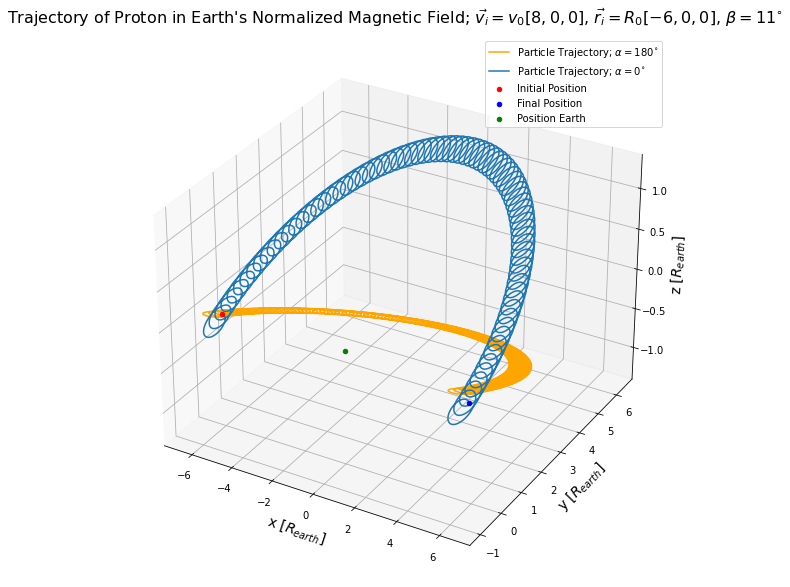
\includegraphics[scale=.4]{Images/protonTrajectories12.png}
    \caption{Trajectories of a proton in earth's magnetic field plotted in 3D. The orientation of the tilt is varied in the two curves. Initial conditions $r_i=R_0[-6,0,0]$, $v_i=v_0[10,0,0]$, $\beta=11^{\circ}$}
    \label{fig:3dTrajectory12}
\end{figure}

\noindent There are two key aspects of the trajectory of the particles: they move in a spiralling motion, and they are deflected around the origin. The spiralling motion is seen to occur perpendicular to the magnetic field, which is due to the cross product in eq. \ref{eq:LorentzForce}. The reason for why the particle does not just move in a circle is because the field becomes weaker as the proton moves away for the origin, meaning its spiral motion gets less sharp and the particle translates. The translation happens perpendicular to the field, and also around the origin because the field continuously accelerates the proton in a spiralling motion such that it keeps a consistent distance to the origin, but translates along the field. The fact that the particle moves along the field is apparent in Figure \ref{fig:planeTrajectory1} since the motion in the $yz$-plane is in one plane perpendicular to the dipole moment. The spiralling motion is only present in the $xz$- and the $xy$-planes.

\begin{figure}[H]
    \centering
    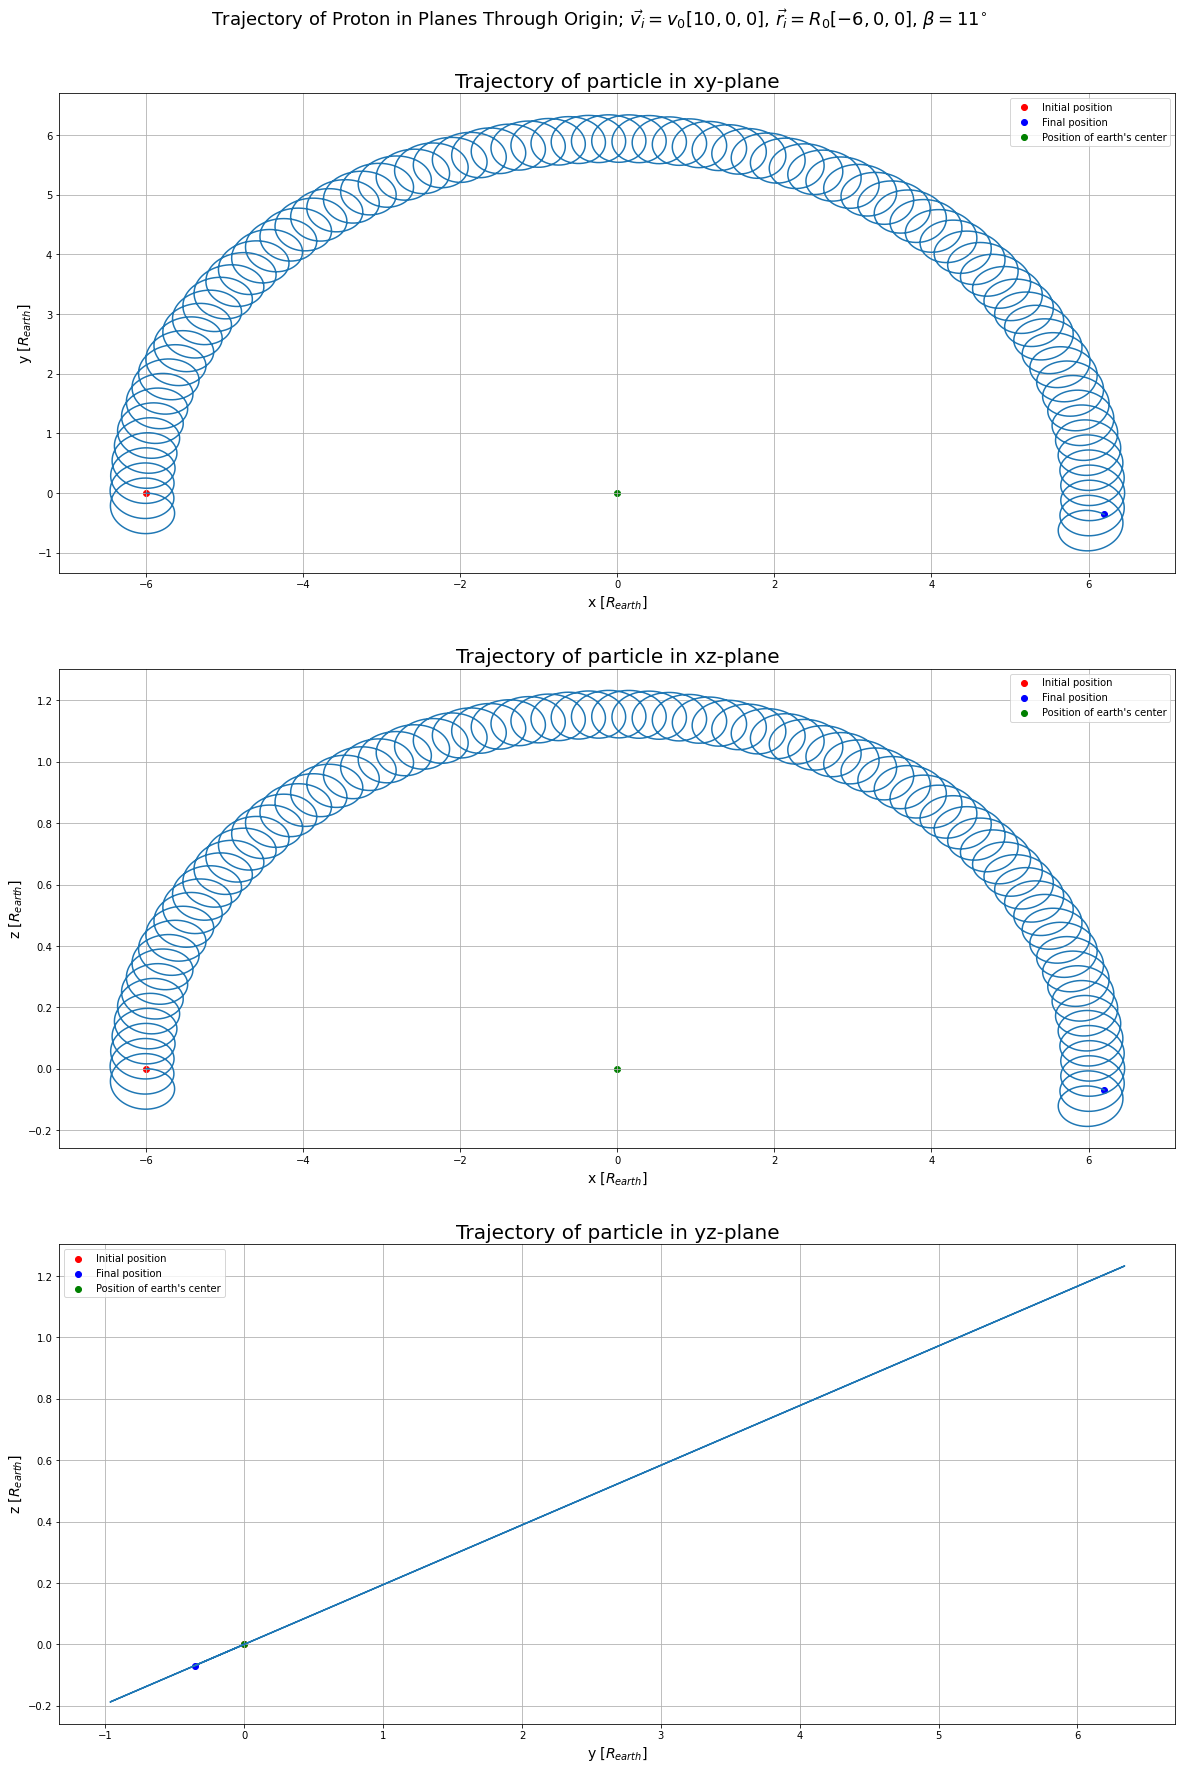
\includegraphics[scale=.20]{Images/trajectoryPlanes1.png}
    \caption{Trajectory of a proton in earth's magnetic field in the various planes through the origin. Initial conditions $r_i=R_0[-6,0,0]$, $v_i=v_0[10,0,0]$, $\beta=11^{\circ}$ and $\alpha=0^{\circ}$}
    \label{fig:planeTrajectory1}
\end{figure}

In Figure \ref{fig:3dTrajectory12} we have plotted two different trajectories; identical initial conditions except one has $\alpha=0^{\circ}$ and one has $\alpha=180^{\circ}$. The effect of this is that the plane of motion for the proton is changed in accord to the direction of the dipole moment; the proton must travel in a plane perpendicular to the field.

\begin{figure}[H]
    \centering
    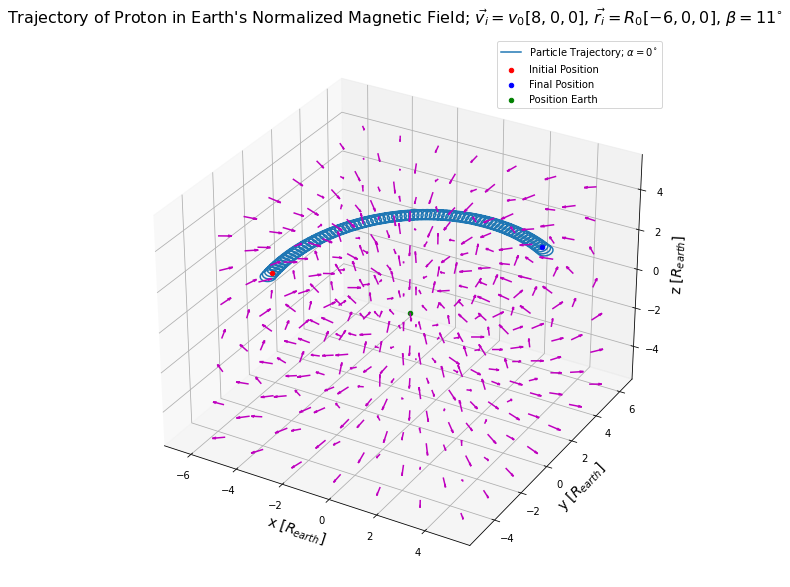
\includegraphics[scale=.4]{Images/protonTrajectory3.png}
    \caption{Trajectory of proton in earth's magnetic field. Initial conditions $r_i=R_0[-6,0,0]$, $v_i=v_0[8,0,0]$, $\beta=11^{\circ}$ and $\alpha=0^{\circ}$}
    \label{fig:3dTrajectory3}
\end{figure}

\noindent The proton in Figure \ref{fig:3dTrajectory3} differs from the others in that the initial velocity is less than those in Figure \ref{fig:3dTrajectory12}. The effect of this lower speed is that the spirals are smaller and that the proton does not travel as far. In Figure \ref{fig:3dTrajectory3} we have in addition to plotting the trajectory also plotted the magnetic field. This is to make it a bit more apparent that the proton moves perpendicular to the field.\\
\\
The last proton trajectory we shall examine is that of a proton which does not start along the $x$-axis. In figures \ref{fig:3dSquiggle} and \ref{fig:squigglyPlane} we see the trajectories of such a proton in 3D and in the $yz$-plane. This trajectory appears much more chaotic, but does have some beautiful symmetries to it. Firstly, the proton is still deflected around the earth. Secondly, the trajectory is still a spiral as seen from above ($xy$-plane). What is interesting though is the fact that the proton seems to oscillate along the direction of the dipole moment. This is the most prominent change that occurs when the proton travels off center.

\begin{figure}[H]
    \centering
    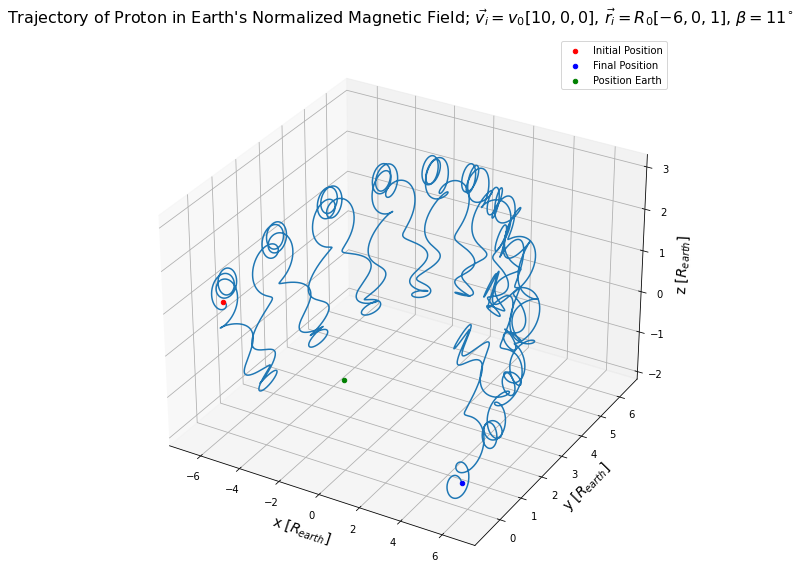
\includegraphics[scale=.4]{Images/squigglyTrajectory.png}
    \caption{Trajectory of proton in earth's magnetic field. Initial conditions $r_i=R_0[-6,0,0]$, $v_i=v_0[8,0,0]$, $\beta=11^{\circ}$ and $\alpha=0^{\circ}$}
    \label{fig:3dSquiggle}
\end{figure}

\begin{figure}[H]
    \centering
    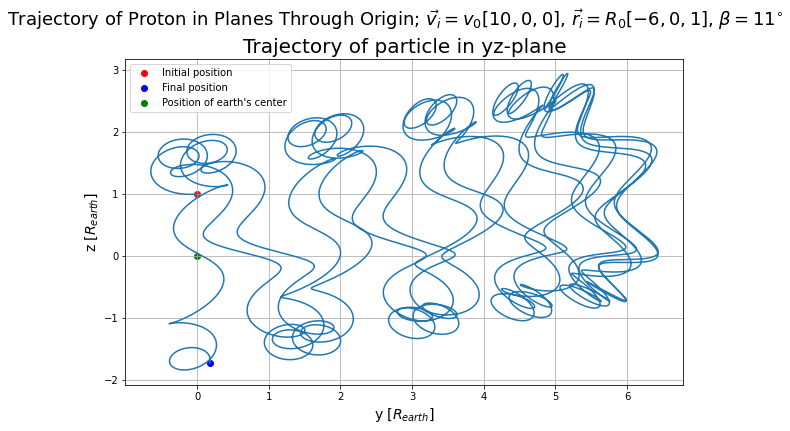
\includegraphics[scale=.4]{Images/squigglyPlane.png}
    \caption{Trajectory of proton in earth's magnetic field in the $yz$-plane. Initial conditions $r_i=R_0[-6,0,0]$, $v_i=v_0[8,0,0]$, $\beta=11^{\circ}$ and $\alpha=0^{\circ}$}
    \label{fig:squigglyPlane}
\end{figure}

\noindent As mentioned in the theory section, the magnetic field does not do any work on the proton, meaning its kinetic energy must remain constant. Change in kinetic energy serves then as an indicator of the accuracy of our simulations. We calculate the relative kinetic energy of a given proton to see how many percent it deviates from the initial kinetic energy. The relative kinetic energy is plotted as a function of time in Figure \ref{fig:kinEnergy3}.

\begin{figure}[H]
    \centering
    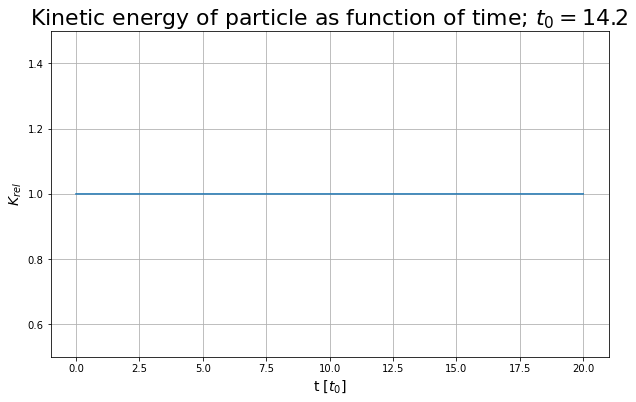
\includegraphics[scale=.4]{Images/KinEnergy3.png}
    \caption{Relative kinetic energy of a proton as a function of time. Initial conditions $r_i=R_0[-6,0,0]$, $v_i=v_0[10,0,0]$, $\beta=11^{\circ}$ and $\alpha=0^{\circ}$}
    \label{fig:kinEnergy3}
\end{figure}

\noindent Figure \ref{fig:kinEnergy3} shows that the relative kinetic energy stays approximately constant to within to $0.0000081\%$, which we can view as an acceptable error. Our calculations are with that very accurate.\\
\\
We remark that the most important effect of the magnetic field of the earth is to shield it from phenomena such as solar winds. In our simulations we see just how it happens and in some sense why. The magnetic field continuously changes the direction of the incoming particles without doing any work and deflects them in a spiralling motion. This all happens because of how magnetic fields interact with moving particles; through a cross product and therefore perpendicular to the direction of motion. A theoretical electric field in place of the magnetic field could be thought to be much less effective at shielding, because it would need to do work to decelerate and scatter the incoming particles.\\
\\
Lastly, it is worth mentioning that this indeed is a very simplified model of the northern lights. Actual solar winds consist of large clouds of particles which in turn interact amongst themselves and produce themselves electromagnetic fields. This is also evident in our plots. The spiralling motion of the protons can be thought of as current carrying loops. Such loops produce a magnetic field, and by the right hand rule one can see in our plots that the protons would produce a magnetic field which would oppose the field of the earth. The solar wind would thus change the magnetic field drastically. In reality, the magnetic field of the earth gets dramatically skewed by solar winds, but do in fact shield the earth similarly to what we have seen in or simulations.\\

\section{Conclusion}
In conclusion, we have used a very simple model in order to simulate the northern light. We approximated the earth's magnetic field by that of a pure magnetic dipole and the solar winds as single protons travelling towards the earth. By numerical solution of the equations of motion for the protons, we found that the protons move in a spiralling trajectory around the earth's center in a plane perpendicular to the magnetic field of the earth. Because the magnetic field exerts a force perpendicular to the direction of motion, the field does no work on the particle. This in turn leaves the kinetic energy of the protons constant. Our simulations show how effectively the magnetic field of the earth shields itself from incoming particles by deflecting them. Though our model is a very simplistic compared to reality, it serves to present the essence of how incoming particles interact with the magnetic field of the earth.

\begin{thebibliography}{9}
\bibitem{griffiths17}
    Griffiths, D. J. (2019). Introduction to electrodynamics. Cambridge University Press.
\bibitem{gitHubRep}
    GitHub Repository with Jupyter Notebook: \url{https://github.com/ingveh/Numerical-Project-Electromagnetic-Theory-Spring2023}

\end{thebibliography}
\end{document}
